Our metadata storage backend implements a modified version of \tfs
to manage all the metadata and small files on disk.
\tfs \cite{TableFS} is a stacked file system which uses another file system
as an object store, and organize all metadata and small files in to a single
on-disk table using a Log-Structured Merge (LSM) tree \cite{ONeil1996}.
The reason of using LSM tree is that it buffers new and changed entries in
memory and translate small random disk writes into large sequential writes.
Therefore LSM tree can reduce random disk seeks effectively, and is a natural
fit for metadata intensive workloads. We decribe the structure of LSM tree
and how LSM tree is used in \tfs to store metadata in greater details
in the following sections.

%\begin{figure}[!ht]
\begin{figure}[t]
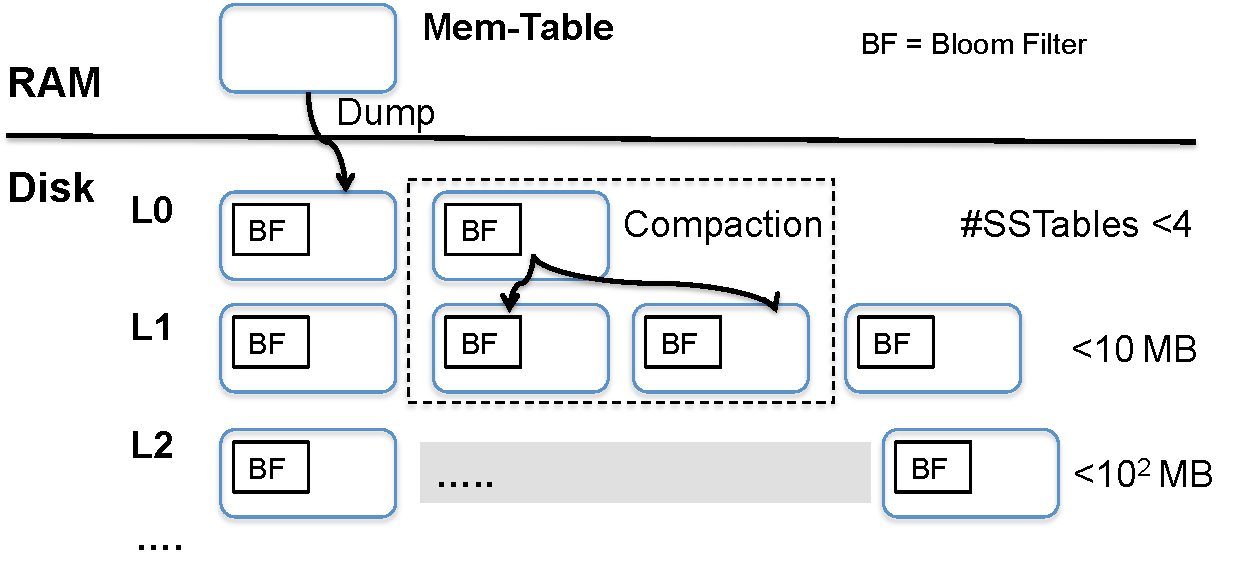
\includegraphics[scale=0.4]{figs/leveldb}
\vspace{10pt}
\caption{\textsf{\footnotesize
LevelDB is an on-disk LSM-tree implementation that represents data in multiple 
files (called SSTables) containing sorted key-value pairs.
SSTables are grouped into different levels with lower-numbered levels
containing more recently inserted key-value pairs.
Finding a specific pair on disk may search up to all SSTables in level-0
and at most one in each higher-numbered level.
Compaction is the process of combining SSTables
by merge sort and moving combined SSTables into higher-numbered levels.
}}
%\vspace{10pt}
\hrule
\label{fig:leveldb}
\end{figure}


\textbf{LSM tree and LevelDB --}
\tfs uses an open-source implementation of LSM tree called LevelDB
\cite{LevelDB}. LevelDB provides a simple key-value store interface,
supporting point query and range query. In LevelDB, by default,
a set of changes are spilled to disk when the total size of modified
entries exceeds 4 MB.  When a spill is triggered, called a
minor compaction, the changed entries are sorted, indexed and written to disk
in a format called an SSTable \cite{BigTable}.  These entries may then be
discarded by the in memory buffer and can be reloaded by searching each SSTable
on disk, possibly stopping when the first match occurs if the SSTables are
searched most recent to oldest.  The number of SSTables that need to be
searched can be reduced by maintaining a Bloom filter\cite{bloomfilter} on each,
but, with time, the cost of finding a record not in memory still increases.
Major compaction, or simply ``compaction",
is the process of combining multiple SSTables
into a smaller number of SSTables by merge sort.

As illustrated in Figure \ref{fig:leveldb},
LevelDB extends this simple approach to further
reduce read costs by dividing SSTables into levels.
In 0-th level, each SSTable may contain entries with any key value,
based on what was in memory at the time of its spill.
The higher-numbered levels of LevelDB's SSTables are
the results of compacting SSTables from their own or lower-numbered levels.
In levels excepth the 0-th level, LevelDB maintains the following invariant:
the key range spanning each SSTable is disjoint from
the key range of all other SSTables at that level.
So querying for an entry in the higher levels
only needs read at most one SSTable in each level.
LevelDB also sizes each of the higher levels differentially:
all SSTables have the same maximum size and
the sum of the sizes of all SSTables at level $L$ will not exceed $10^L$ MB.
This ensures that the number of level grows
logarithmically with increasing numbers of entries.

~\\
\textbf{Table schema -- }
\tfs aggregates directory entries,
inode attributes and small files into one LSM tree
with an entry for each file and directory.
To translate the hierarchical structure of file system namespace
into key-value pairs, the 224-bit key is chosen to consist of
the 64-bit inode number of a entry's parent directory
and a 160-bit SHA-1 hash value of its filename string
(final component of its pathname).
The value of an entry contains the file's full name and inode attributes,
such as inode number, ownership, access mode, file size, timestamps (\textit{struct stat} in Linux).
For small files with size less than $T$, the value field also contains the file's data.
For large files, its file data is replaced by a symbolic link
that points to the actual file object in the underlying cluster file system.

%\begin{figure}[!ht]
\begin{figure}[t]
\centering
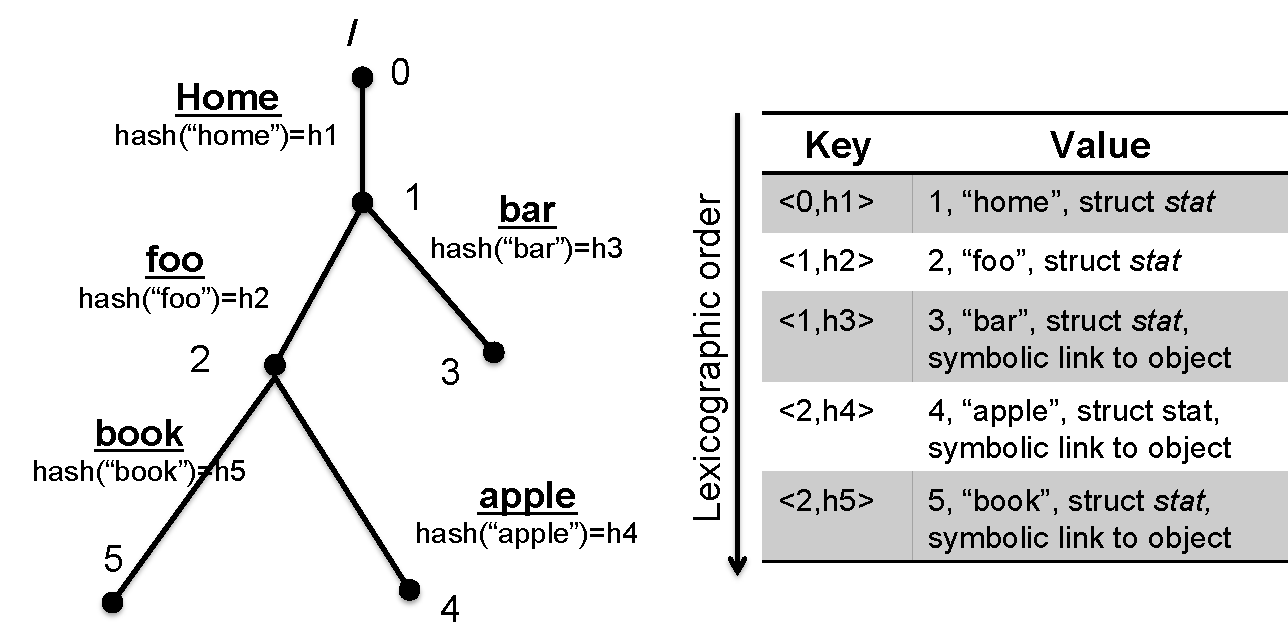
\includegraphics[scale=0.4]{figs/schema}
\vspace{10pt}
\caption{\textsf{\footnotesize
An example illustrating a table schema for \tfs
to store metadata and file data as key-value pairs.}}
%\vspace{10pt}
\hrule
\label{fig:schema}
\end{figure}

Figure \ref{fig:schema} shows an example of representing
a sample file system's metadata into one table.
Embedding the inode number of parent directory into the key
helps with resolving the pathname.
Traversing the user's directory tree
only involves constructing a search key by concatenating the inode
number of current directory with the hash of
next component name in the pathname.
Another benefit is that all the entries in the same directory have rows that
share the same first 64 bits in their the table's key.
For $readdir$ operations, once the inode number
of the target directory has been retrieved,
a scan sequentially lists all entries having
the directory's inode number as the first 64 bits of their table's key.

Previous evaluation \cite{TableFS} has shown using \tfs schema with \ldb backend
can greatly improve metadata performance of the local file system.
Figure \ref{graph:ldb-singlenode} is taken from the original \tfs paper,
which compares the instantaneous throughput of FUSE-based \tfs
with three Linux file systems: Ext4 \cite{Ext4}, XFS \cite{XFS}, and
Btrfs \cite{BTRFS}.
The workload is to create 100 million zero-length files in a single directory.
All systems perform well at the beginning of the test, but the file create
throughput drops gradually for all systems.
Btrfs suffers the most serious throughput drop, slowing down to 100 operations
per second.
\tfs, however, maintains a more steady performance
with an average speed of 2,200 operations per second respectively,
\textit{and is 10X faster than all other tested file systems.}

\begin{figure}[t]  %%%%%%%%%%%%%%%%%%%%%%%
\centerline{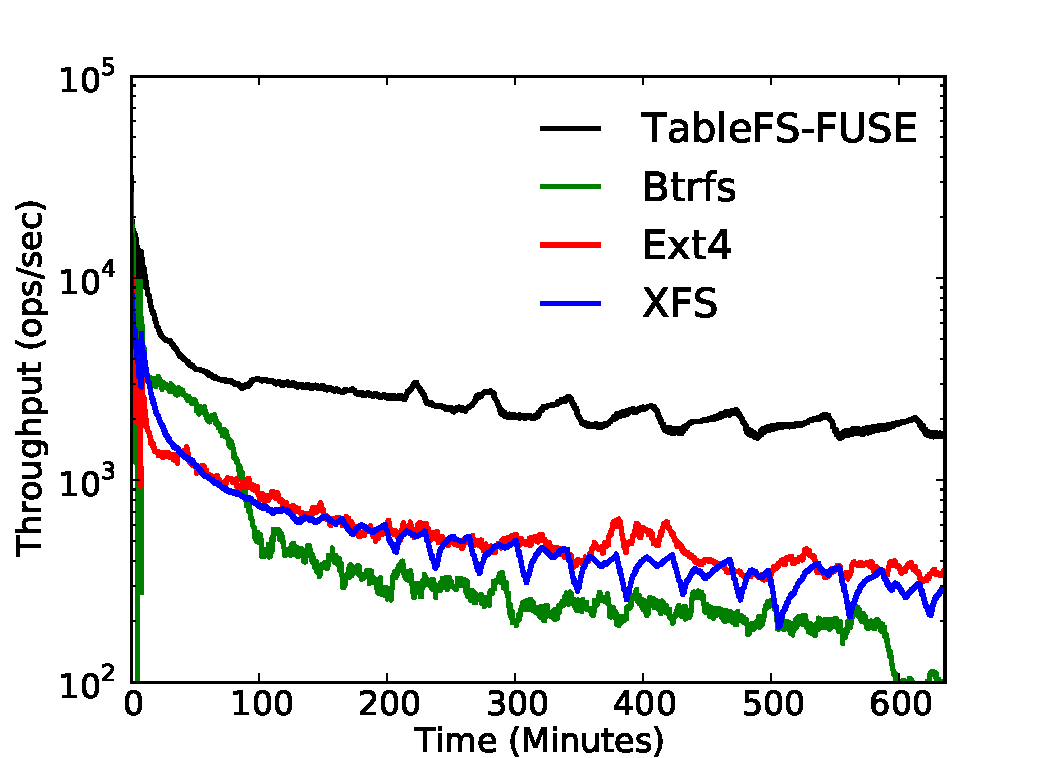
\includegraphics[scale=0.5]{./figs/ldb_insertrate_onenode}}
\vspace{10pt}
\caption{\textsf{\footnotesize
This graph (from prior work \cite{TableFS}) shows
that the performance of single-node \tfs with FUSE is 10X faster than modern Linux
filesystems. The workload is to create 100 million zero-length files in one directory.
X-axis only shows the time until \tfs finished all insertions because the other
file systems were much slower. Y-axis has a logarithmic scale.}
}
%\vspace{10pt}
\hrule 
\label{graph:ldb-singlenode}
\end{figure}       %%%%%%%%%%%%%%%%%%%%%%%
